%Definiciones previas y uso de paqueterías
\documentclass[12pt]{article}
\usepackage[utf8]{inputenc}
\usepackage{graphicx} % Required for inserting images
\usepackage[spanish]{babel}
\usepackage{geometry}
\usepackage{setspace}
\usepackage{sectsty} %Para cambiar el tamaño de diferentes secciones

%Para el formato APA
\usepackage{apacite}

%Márgenes
\newgeometry{left=1in, right=1in, top=1in, bottom=1in}

\begin{document}

%Haciendo portada
\begin{titlepage}
\centering
{\bfseries\Large Universidad Nacional Mayor de San Marcos\par}
{\large Universidad del Perú, Decana de América\par}
{\scshape\Large Facultad de Ingeniería de Sistemas e Informatica\par}
{\scshape\Large Escuela Profesional de Ingeniería de Sistemas\par}
\vspace{0.5cm}
{
\includegraphics[width=0.40\textwidth]{imagenes/1 escudo san marcos.png}\par}
\vspace{0.5cm}
{\bfseries\large Informe Proyecto Final

Nombre del proyecto\par}
\vspace{0.05cm}
{\bfseries\large Grupo N.º 10\par}
\vspace{0.5cm}


{\bfseries\large Asigntatura:}
{\large Programación de Computadoras I\par}
\vspace{0.5cm}

{\bfseries\large Docente:}
{\large Guerra Grados, Luis Angel\par}
\vspace{0.5cm}

{\bfseries\large Integrantes:\par}
{\large
\begin{center}
\begin{tabular}{c@{\hspace{2cm}}c}
Cardenas Huaman, Ariana Milagros & 24200000 \\
Cruz Ramos, Alysson Kiara    	& 24200000 \\
Flores Hoyos, Mathias Pavel Diego & 24200014 \\
Meza Dalguer, Anyel Giuliana 	& 24200000 \\
\end{tabular}
\end{center}}

\vspace{1in}

{\bfseries\large Lima, Perú\par}
{\bfseries\large 2025-I\par}
\end{titlepage}
%Fin de portada

%Cuerpo del documento
	%Tamaño de fuente 12 e interlineado 1.5
{\fontsize{12}{18}\selectfont % Fuente 12pt, interlineado 1.5x
\doublespacing
    
	% Cambiar tamaño de títulos para que escalen con 12pt
\sectionfont{\Large} 	% Sección: tamaño Large (aprox 14.4pt)
\subsectionfont{\large} % Subsección: tamaño large (12pt)
\subsubsectionfont{\normalsize}
%Índice


%Introducción
\section{Introducción}
El reconocimiento facial automatizado ha revolucionado la forma en que interactuamos con la tecnología, ofreciendo soluciones innovadoras en diversos campos. Este proyecto explora el desarrollo de un sistema de identificación facial desarrollado en el lenguaje de programación de alto nivel, Python, donde el elemento clave reside en el proceso de entrenamiento de la máquina para reconocer patrones faciales únicos. A través de algoritmos de aprendizaje automático, el sistema adquiere la capacidad de analizar y memorizar las características distintivas de cada rostro, transformando complejos rasgos faciales en representaciones matemáticas que permiten comparaciones rápidas y eficientes.  

El enfoque adoptado prioriza la simplicidad y el rendimiento, utilizando técnicas fundamentales de procesamiento de imágenes que garantizan un funcionamiento óptimo. La conversión a escala de grises se incorpora como un paso adicional de optimización, ayudando a reducir la complejidad computacional sin comprometer la capacidad de reconocimiento.

Si bien existen limitaciones inherentes relacionadas con condiciones variables de iluminación o ángulos no frontales, los resultados demuestran que es posible construir un reconocedor facial efectivo utilizando herramientas accesibles. Este documento detalla el proceso completo de entrenamiento del modelo, desde la preparación de los datos hasta la implementación final, ofreciendo una visión clara de cómo la inteligencia artificial puede aplicarse para resolver problemas concretos en la vida cotidiana. Más allá de los aspectos técnicos, el proyecto ilustra el potencial de estas tecnologías para crear sistemas de identificación personalizados, abriendo posibilidades interesantes para desarrollos futuros con mayor grado de sofisticación.


%Planteamiento del problema
\section{Planteamiento del problema}
En el contexto de la Universidad Nacional Mayor de San Marcos, existe una problemática significativa en el control de accesos que afecta tanto la seguridad como la eficiencia institucional. El sistema actual, basado en identificación mediante carnets físicos, presenta múltiples limitaciones que comprometen la integridad de las instalaciones y la agilidad operativa. Simultáneamente, los procesos manuales de verificación ocasionan congestiones en los accesos principales, particularmente durante horas de alta circulación de personas, retrasando la movilidad de estudiantes y docentes hacia sus actividades académicas.Esta situación demanda urgentemente una solución tecnológica que modernice los procesos de identificación, garantizando simultáneamente mayor seguridad y eficiencia operativa.

La implementación de un sistema de reconocimiento facial se presenta como la alternativa óptima para superar estos desafíos. Esta innovación reforzaría sustancialmente la seguridad institucional al eliminar los riesgos de suplantación asociados a documentos físicos, mediante la verificación biométrica en tiempo real contra una base de datos centralizada. La tecnología permitiría agilizar significativamente los flujos de acceso, eliminando cuellos de botella en los puntos de ingreso y facilitando el registro automático de asistencia con fines académicos y estadísticos.

Desde la perspectiva ambiental, el proyecto promoverá la sostenibilidad al reducir el consumo de materiales plásticos y papel utilizados en la producción de carnets físicos o tomas de asistencia. Los usuarios se verán beneficiados en comodidad y autonomía al liberarse de la necesidad de portar documentos físicos, eliminando los problemas asociados a su pérdida u olvido. La solución está diseñada con capacidad de escalamiento, permitiendo su adaptación a diversos escenarios institucionales más allá del ámbito universitario, incluyendo colegios, centros médicos y empresas privadas que requieran sistemas de control de acceso seguros y eficientes.

Esta iniciativa no solo modernizará la gestión de accesos en la UNMSM, sino que establecería un precedente tecnológico para otras instituciones educativas nacionales. Al implementar un sistema biométrico de vanguardia, la universidad reforzaría su posición como institución líder en innovación tecnológica, al tiempo que contribuiría a la transformación digital del país con un modelo sostenible, seguro y eficiente.


%Objetivos
\section{Objetivos}
\subsection{General}
Desarrollar e implementar un sistema de reconocimiento facial para el control de acceso en las instalaciones de la Universidad Nacional Mayor de San Marcos, que mejore la seguridad institucional, optimice los procesos de ingreso y sustituya los métodos tradicionales de identificación física, contribuyendo a la modernización tecnológica de la universidad.
\subsection{Específicos}
Automatizar los procesos de control de acceso y registro de asistencia, eliminando la dependencia de carnets físicos y reduciendo los tiempos de verificación en los puntos de ingreso principales, con capacidad de generar reportes automatizados para la gestión administrativa.

Diseñar una solución escalable y adaptable que pueda extenderse a diferentes facultades y dependencias de la universidad, con potencial para ser implementado en otras instituciones educativas o centros que requieran sistemas de control de acceso seguros y eficientes.


%Marco Teórico
\section{Marco Teórico}
wasaaa


%Metodología
\section{Metodología}
El desarrollo del sistema de reconocimiento facial se basa en un enfoque estructurado que combina técnicas de procesamiento de imágenes y aprendizaje automático. A continuación, se detallan las etapas clave del proceso:
\subsection{Captura de imágenes}
\begin{itemize}
	\item Opción 1: Carga de video
	\begin{itemize}
    	\item Los usuarios pueden cargar un archivo de video existente. El sistema extrae los frames del video y detecta automáticamente los rostros presentes en cada frame. Cada rostro detectado se almacena como una imagen individual etiquetada con un código único proporcionado por el usuario.
	\end{itemize}
	\item Opción 2: Grabación en tiempo real
	\begin{itemize}
    	\item Los usuarios pueden activar la cámara web integrada. Al presionar la tecla 'p', el sistema captura los frames en tiempo real, detecta los rostros y los almacena con el código único correspondiente. Este método es ideal para registros rápidos y directos.
	\end{itemize}
\end{itemize}

\subsection{Procesamiento de imágenes}
\begin{itemize}
	\item Conversión a escala de grises: Las imágenes se convierten a escala de grises para reducir la complejidad computacional y mejorar la eficiencia del algoritmo de reconocimiento.
	\item Redimensionamiento: Todas las imágenes se estandarizan a un tamaño fijo (200 x 200 píxeles) para garantizar consistencia en el entrenamiento del modelo.
	\item Detección de rostros: Se utiliza el clasificador Haar Cascade para identificar y extraer regiones de interés (rostros) de cada frame.
\end{itemize}

\subsection{Entrenamiento del modelo}
\begin{itemize}
	\item Algoritmo Eigenfaces: Se emplea el método Eigenfaces, que utiliza el análisis de componentes principales (PCA) para reducir la dimensionalidad de los datos y capturar las características faciales más significativas.
	\item Proceso de entrenamiento: Las imágenes preprocesadas y sus etiquetas correspondientes se utilizan para entrenar el modelo. El sistema genera un archivo XML que contiene los patrones aprendidos.

\end{itemize}

\subsection{Prueba y reconocimiento}
\begin{itemize}
	\item Detección en tiempo real: El sistema utiliza la cámara web para capturar frames y detectar rostros en tiempo real.
	\item Comparación con el modelo: Cada rostro detectado se compara con los patrones almacenados en el modelo entrenado. El sistema devuelve el código asociado al rostro reconocido junto con un nivel de confianza.
	\item Visualización: Los resultados se muestran en una ventana que incluye un rectángulo alrededor del rostro detectado y la información de identificación.
\end{itemize}

\subsection{Interfaz de usuario}
\begin{itemize}
	\item Menú interactivo: El sistema ofrece un menú con opciones para cargar videos, grabar nuevos registros, entrenar el modelo y probar el reconocimiento, facilitando la interacción con el usuario
\end{itemize}

{\large Ventajas del enfoque\par}
\begin{itemize}
	\item Eficiencia: El uso de técnicas de preprocesamiento y algoritmos optimizados garantiza un rendimiento rápido incluso en hardware básico.
	\item Accesibilidad: La implementación en Python con bibliotecas como OpenCV hace que el sistema sea fácil de entender y modificar.
	\item Escalabilidad: La estructura modular permite adaptar el sistema a diferentes entornos, como control de acceso en aulas, laboratorios o eventos institucionales.
\end{itemize}


%Desarrollo del proyecto
\section{Desarrollo del proyecto}
Waaaaasssa


%Resultados
\section{Resultados}
\subsection{Esto es un ejemplo}
Sed hendrerit, nulla quis sollicitudin imperdiet, velit leo imperdiet massa, et gravida neque magna vitae ex. Quisque maximus, elit vitae pellentesque aliquet, eros leo sagittis tellus, vitae maximus dui nulla sed mi. Curabitur tincidunt nibh id lectus porttitor porttitor. Vivamus in sapien id magna elementum mattis eu et massa. Aenean volutpat metus at ante consectetur lacinia. Fusce ante dui, mattis sit amet maximus at, imperdiet quis erat. Sed ultricies arcu in mauris aliquam convallis \cite{rivera2022implementacion}. \bigskip

Sed hendrerit, nulla quis sollicitudin imperdiet, velit leo imperdiet massa, et gravida neque magna vitae ex. Quisque maximus, elit vitae pellentesque aliquet, eros leo sagittis tellus, vitae maximus dui nulla sed mi. Curabitur tincidunt nibh id lectus porttitor porttitor. Vivamus in sapien id magna elementum mattis eu et massa. Aenean volutpat metus at ante consectetur lacinia. Fusce ante dui, mattis sit amet maximus at, imperdiet quis erat. Sed ultricies arcu in mauris aliquam convallis. \bigskip

%Insertar imagen
\begin{figure}[h]
	\centering
	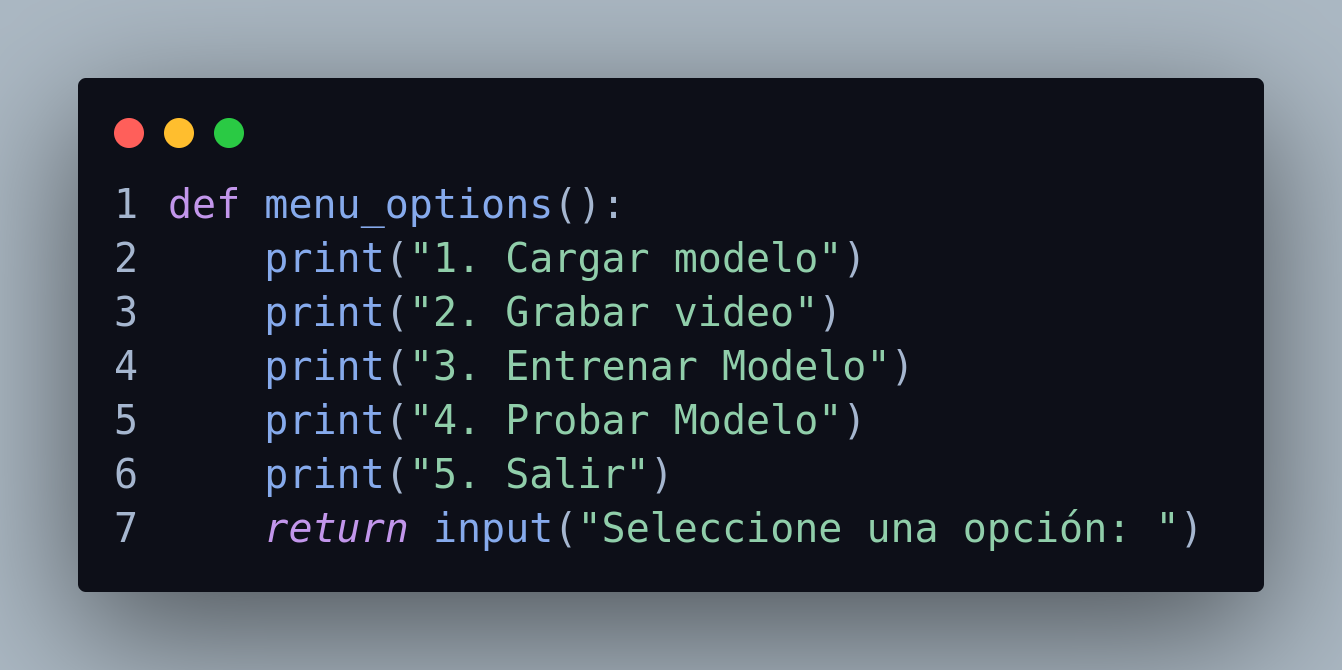
\includegraphics[width=0.85\textwidth]{imagenes/code.png}
	\caption{Menú de opciones}
	\label{fig_1}
\end{figure}



Sed hendrerit, nulla quis sollicitudin imperdiet, velit leo imperdiet massa, et gravida neque magna vitae ex. Quisque maximus, elit vitae pellentesque aliquet, eros leo sagittis tellus, vitae maximus dui nulla sed mi. Curabitur tincidunt nibh id lectus porttitor porttitor. Vivamus in sapien id magna elementum mattis eu et massa. Aenean volutpat metus at ante consectetur de la fig. \ref{fig_1} lacinia. Fusce ante dui, mattis sit amet maximus at, imperdiet quis erat. Sed ultricies arcu in mauris aliquam convallis. \bigskip


%Conclusiones y recomendaciones
\section{Conclusiones y recomendaciones}
bbbbbbbbbbbb


%Anexos
\section{Anexos}
bbbbbbbbbbbbbbb


%Bibliografía
\bibliographystyle{apacite}
\bibliography{bibliografia.bib}

}
%Fin del cuerpo del documento
\end{document}
